\noindent Η ανάλυση των περισσότερων μεθόδων και τεχνικών βελτιστοποίησης που χρησιμοποιήσαμε στα πλαίσια της εργασίας έχει ήδη αναφερθεί στα προηγούμενα ερωτήματα. Στη συνέχεια γίνεται μία σύντομη επισκόπηση του τρόπου με τον οποίο έγινε η παραλληλοποίηση στη GPU του κώδικα του τρίτου ερωτήματος. 

\noindent Στο συγκεκριμένο ερώτημα υπολογίζεται το μητρώο συνδιακύμανσης ενός αρχικού μητρώου μεγέθους \mbox{M X N}. Ο υπολογισμός αυτός γίνεται σε τρία βήματα:

\begin{enumerate}
    \item \textbf{Mean Calculation:} Για κάθε στήλη του μητρώου Α υπολογίζεται ο μέσος όρος των στοιχείων της στήλης.
    
    \item \textbf{Matrix Centering:} Από κάθε στοιχείο κάθε στήλης του μητρώου αφαιρεί τον μέσο όρο της αντίστοιχης στήλης που υπολογίστηκε στο προηγούμενο βήμα.
    
    \item \textbf{Covariance Matrix Calculation:} Πολλαπλασιάζεται το μητρώο που υπολογίστηκε στο προηγούμενο βήμα με το ανάστροφό του. Επειδή το αποτέλεσμα που προκύπτει είναι συμμετρικό μητρώο, αρκεί ο υπολογισμός είτε του άνω είτε του κάτω τριγωνικού μέρους του.
    
    
\end{enumerate}

\subsection*{CUDA-naïve implementation}
\addcontentsline{toc}{subsection}{CUDA-naïve implementation}

\noindent Αρχικά προχωρήσαμε στην απλούστερη δυνατή μορφή παραλληλοποίησης του κώδικα που μας δίνεται, δημιουργώντας έναν υπολογιστικό πυρήνα για κάθε ένα από τα βήματα του υπολογισμού όπως αυτά αναφέρθηκαν παραπάνω. Επίσης δημιουργήθηκε και μία συνάρτηση wrapper η οποία αναλαμβάνει να υπολογίσει τις κατάλληλες παραμέτρους και να καλέσει κάθε kernel.

\begin{enumerate}
    \item \textbf{\texttt{\textunderscore\textunderscore global\textunderscore\textunderscore\  void mean\textunderscore kernel(double *mean\textunderscore d, double *data\textunderscore d)}}
    
    \item \textbf{\texttt{\textunderscore\textunderscore global\textunderscore\textunderscore\  void reduce\textunderscore kernel(double *mean\textunderscore d, double *data\textunderscore d)}}
    
    \item \textbf{\texttt{\textunderscore\textunderscore global\textunderscore\textunderscore\  void covar\textunderscore kernel(double *symmat\textunderscore d, double *data\textunderscore d)}}
    
    \item \textbf{\texttt{\textunderscore\textunderscore host\textunderscore\textunderscore\  void calculate\textunderscore on\textunderscore GPU(...) // wrapper function}}
\end{enumerate}

Επόμενο βήμα είναι ο έλεγχος της ορθότητας των υπολογισμών ώστε να διαπιστώσουμε ότι το πρόγραμμα μας παράγει τα επιθυμητά αποτελέσματα. Για τον λόγο αυτό πέρα από την εγγραφή των αποτελεσμάτων στα αρχεία cpu.out και gpu.out έχει δημιουργηθεί η συνάρτηση \textittt{\textit{compareResults()}} η οποία συγκρίνει μεταξύ τους τα στοιχεία που παράχθηκαν στην CPU και την GPU και μετρά πόσα από αυτά διαφέρουν πάνω από ένα προκαθορισμένο ποσοστό σφάλματος. Η ιδέα αυτή προέρχεται από τον τρόπο με τον οποίο γίνεται η σύγκριση των αποτελεσμάτων στην υλοποίηση των PolyBench benchmarks για GPU όπως αυτά φαίνονται \href{http://web.cse.ohio-state.edu/~pouchet.2/software/polybench/GPU/index.html}{εδώ} και στην εργασία \cite{polybench}.


\subsection*{Βελτιστοποίηση}
\addcontentsline{toc}{subsection}{Βελτιστοποίηση}

\noindent Αφού επιβεβαιώσαμε την ορθότητα των υπολογισμών έγινε η βελτιστοποίηση του παράλληλου κώδικα. Επιτύχαμε πολύ μεγάλη εξοικονόμηση χρόνου με την χρήση καταχωρητών για την αποθήκευση των ενδιάμεσων αποτελεσμάτων. Με αυτόν τον τρόπο αντί να προσπελαύνεται πολλαπλές φορές η global memory απο κάθε thread, χρησιμοποιείται μία τοπική μεταβλητή για την αποθήκευση του αποτελέσματος και στην συνέχεια αυτό εγγράφεται στην global memory όταν έχει ολοκληρωθεί ο υπολογισμός του.

\pagebreak

\subsection*{Αποτελέσματα}
\addcontentsline{toc}{subsection}{Αποτελέσματα}

\noindent Παρακάτω συγκεντρώνονται τα αποτελέσματα επαναλαμβανόμενων εκτελέσεων του προγράμματος για διαφορετικά μεγέθη εισόδου.

\begin{center}
    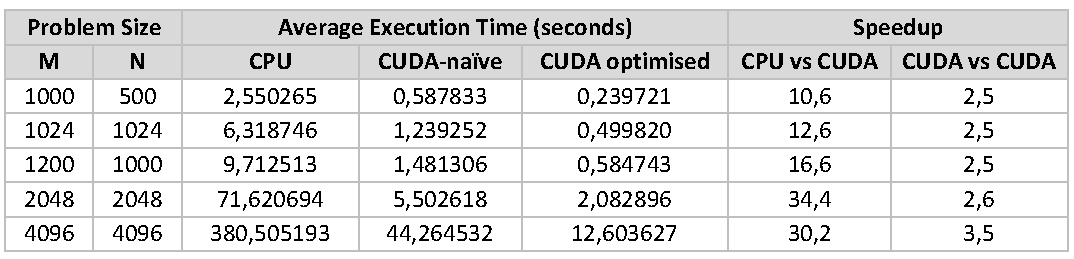
\includegraphics[scale=0.85]{./figures/3_covar/covar}
\end{center}

\noindent Το πρώτο speedup που υπολογίζεται αφορά την επιτάχυνση που δίνει ο βελτιωμένος κώδικας σε σχέση με την σειριακή εκτέλεση στη CPU. Το δεύτερο speedup αναφέρεται στην επιτάχυνση που έδωσαν οι βελτιστοποιημένοι cuda kernels σε σχέση με την naive εκδοχή τους. 

\subsection*{Συμπεράσματα}
\addcontentsline{toc}{subsection}{Συμπεράσματα}

Το πρώτο που παρατηρούμε είναι ότι η χρήση καταχωρητών αντί για προσπέλαση της global memory είναι απο μόνη της ικανή να μας δώσει πολύ μεγάλη βελτίωση του χρόνου εκτέλεσης. Επίσης γίνεται φανερό ότι όσο μεγαλώνει το μέγεθος του προβλήματος, τόσο μεγαλύτερο speedup επιτυγχάνεται που όμως μετά από ένα σημείο παραμένει σχετικά σταθερό.

\begin{center}
    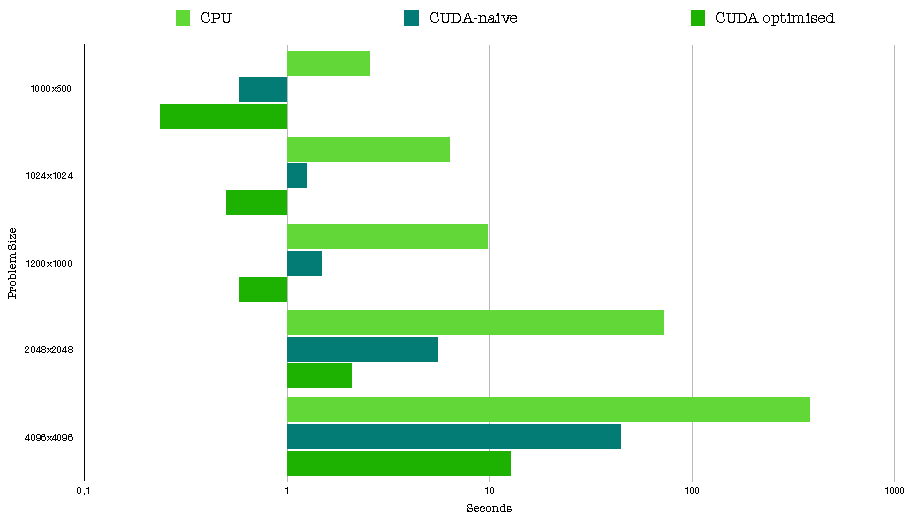
\includegraphics[scale=1]{./figures/3_covar/diag}
\end{center}